We compared the hidden Markov development model to
the latent change-point and two-step models 
using two sets of data.

Firstly, the models were fit to 200 industry
paid loss triangles from \cite{meyers2015}, 50 triangles
for the four lines of business: private passenger auto (PP),
workers compensation (WC), commerical auto (CA), and
other occurrence (i.e. general) liability (OO).
We removed three triangles with zero loss values first,
one from the CA dataset and two from the OO dataset.
Each triangle covered 10 years of historical
accident and development periods, amenable to partitioning
into an upper diagonal of training data,
$\mathcal{Y}$, and lower diagonal of test data,
$\tilde{\mathcal{Y}}$.
As these are yearly triangles, and have been
chosen for previous model validation exercises \citep{meyers2015},
it is reasonable to assume that the losses at development
period 10 are close to ultimate.
For the two-step approach, we inspected the
mean and standard deviations of the empirical
link ratios across triangles (shown in Figure
\ref{fig:industry-atas}), and selected
$\tau = 6$ and $\bm{\rho} = (4, 10)$. These
were chosen given
that the link ratios showed smooth patterns
of decay from approximately development period
4 onwards, and the
triangles were close, on average, to their values
at period 10 by development period $\tau = 6$.

When fitting the models to industry triangles,
a small number of models
produced
very large posterior predictions on out-of-sample
data, which numerically overflowed. The multiplicative
autoregressive nature of typical loss development models
mean that large predictions at one
time point can quickly compound to unrealistic and
computationally-unstable values. For this reason,
we capped the predictions at 100 times the
maximum value across the training and test data
for each triangle.

\begin{figure}
    \centering
    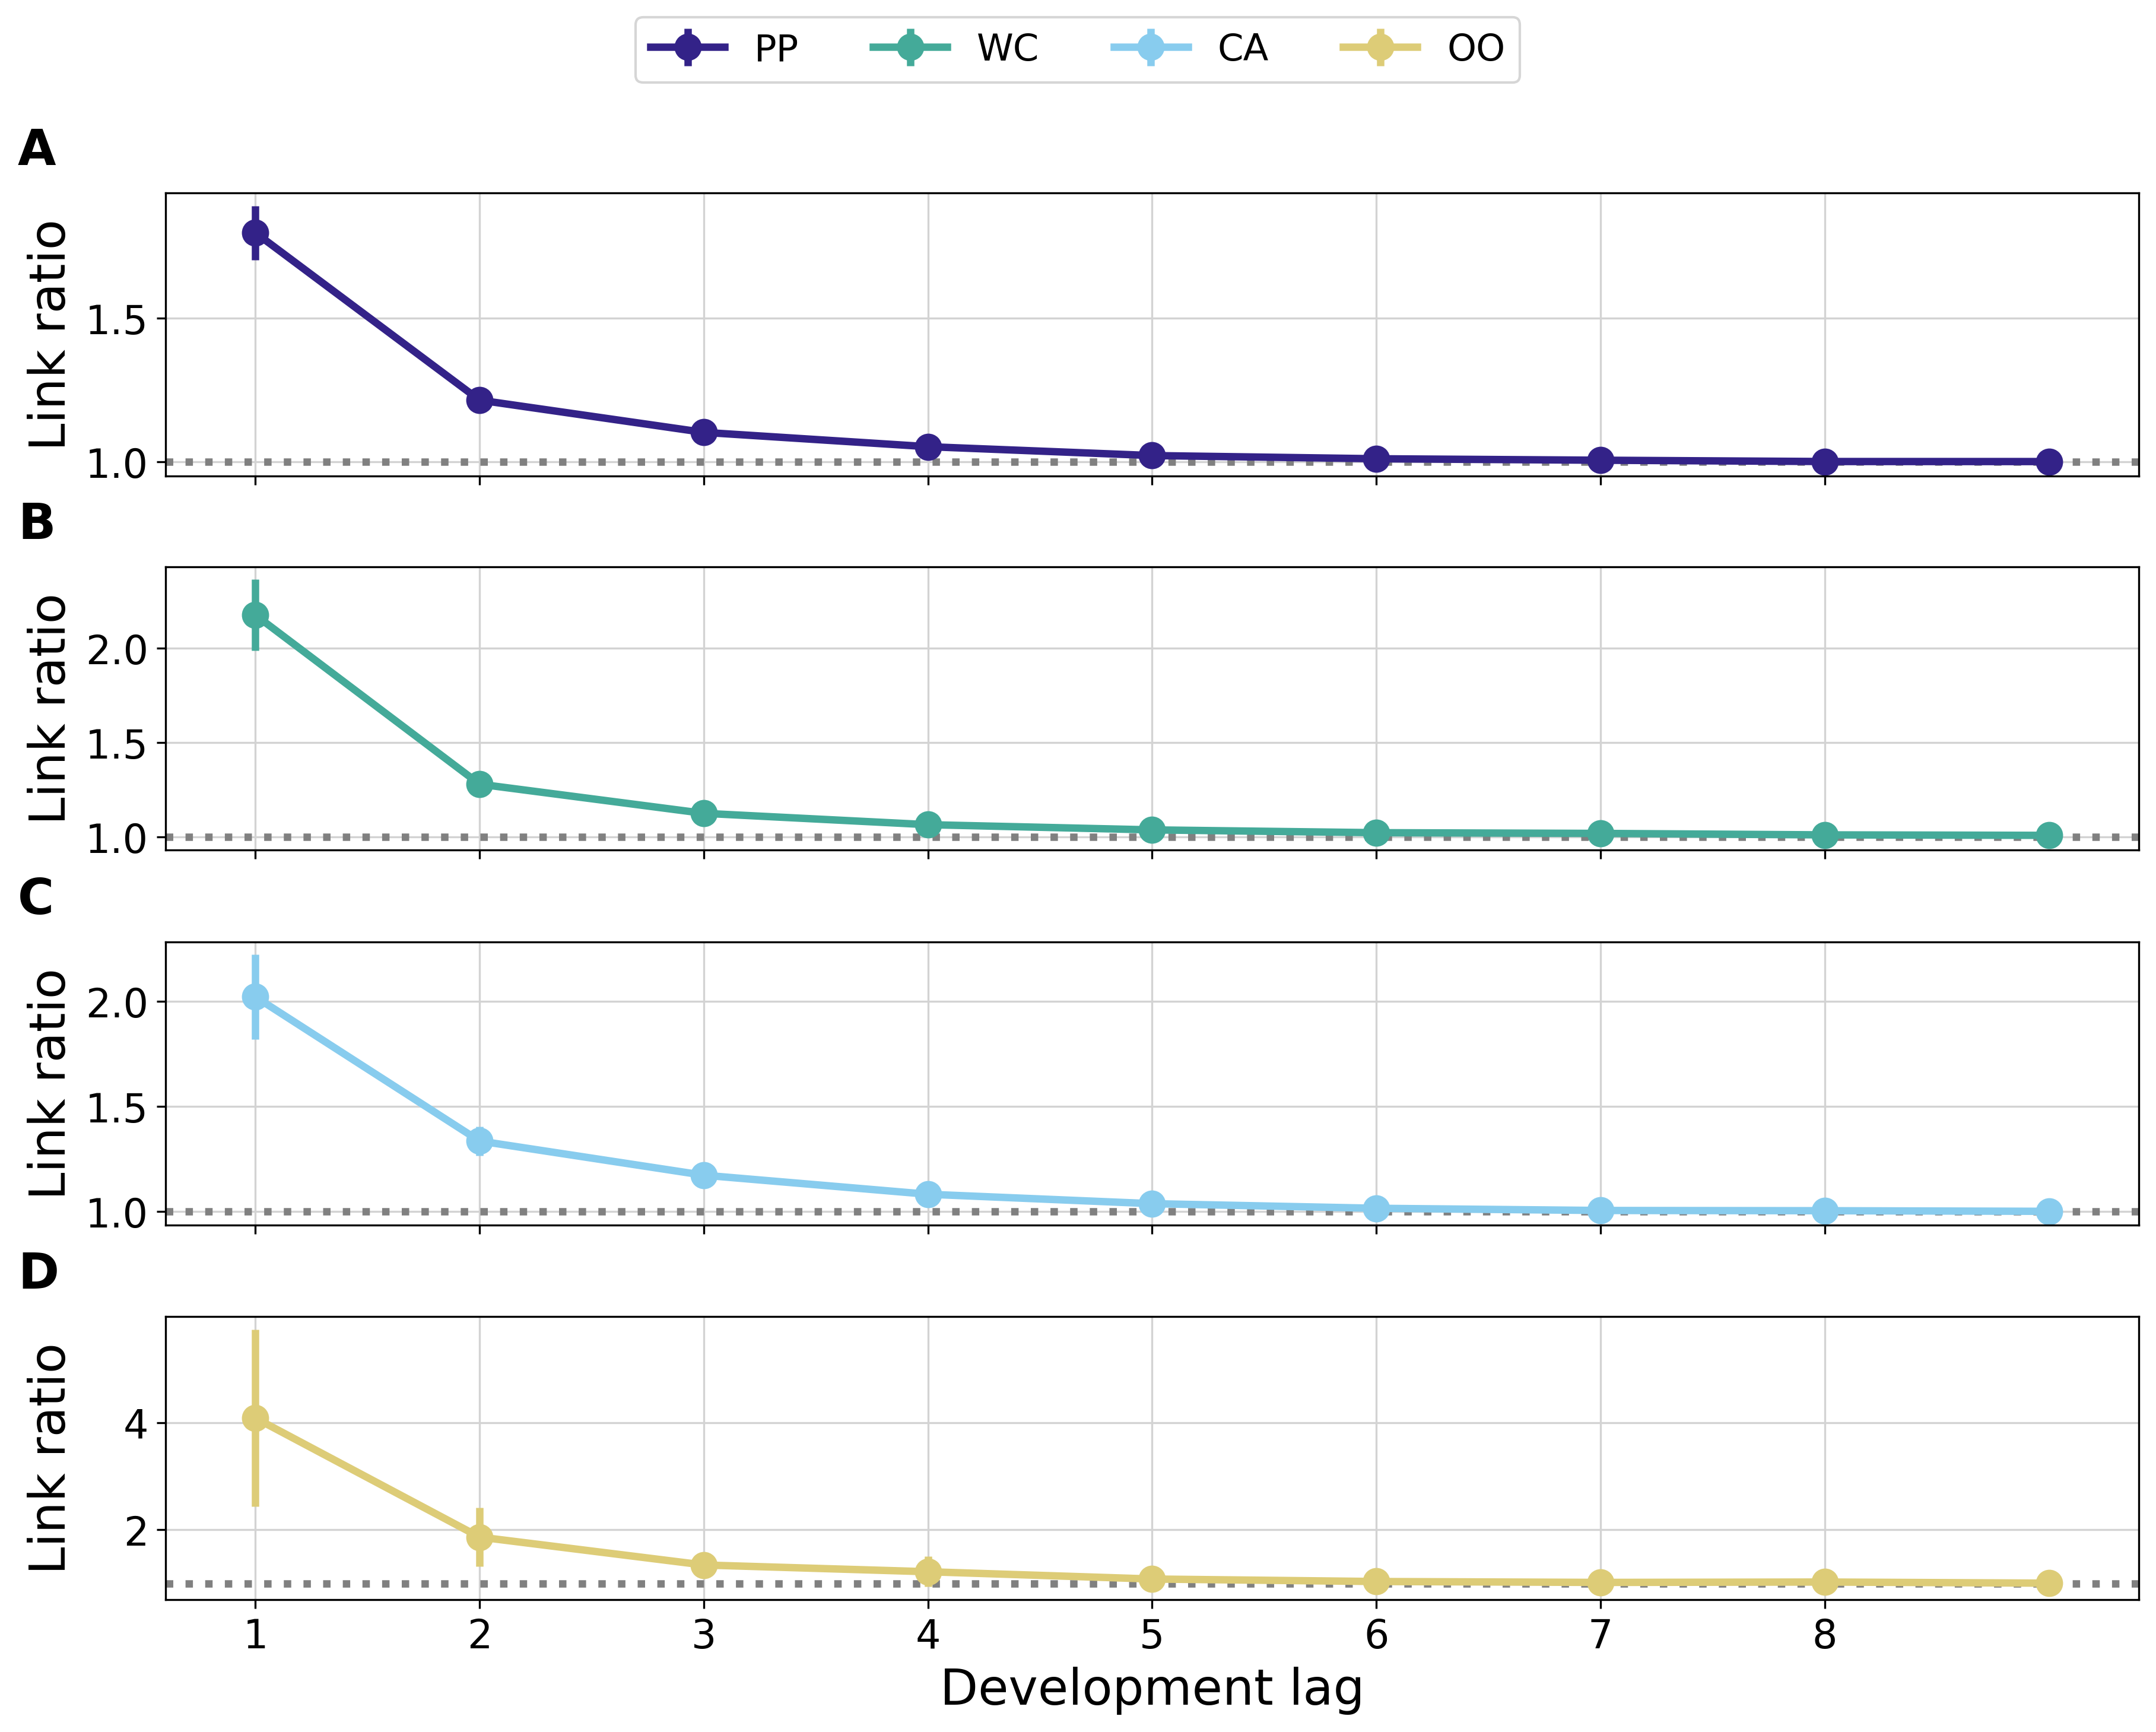
\includegraphics[scale=0.4]{\figures/atas.png}
    \caption{
        The empirical link ratios by line of business 
		(panels A-D) in
        the \cite{meyers2015} dataset.
        Points indicate the mean across triangles,
        and vertical line segments show 2 standard
        deviations.
    }
	\label{fig:industry-atas}
\end{figure}

Secondly, we used 5
triangles presented in the
relatively recent literature on key
papers on loss development
modelling,
including tail development, that provide more
historical data than the industry triangles:
the long-tailed liability and short-tailed property 
quarterly triangles from medium-size insurers
in \cite{balona2022}, the annual liability triangle in \cite{merz2015},
the Swiss annual liability triangle from \cite{gisler2009},
and the annual liability triangle in \cite{verrall2012}.
These triangles had between 17 and 22 periods of
data. For each triangle, we used the latest diagonal as the
test dataset to evaluate predictive performance.
For the two-step modelling approach, we chose the
$\tau$ and $\bm{\rho}$ constants
by visual inspection of the empirical link ratios,
selecting $(4, 4, 4, 4, 11)$ for $\tau$ values
for each triangle,
and $[(4, 16), (3, 20), (3, 21), (3, 16), (10, 21)]$
for $\bm{\rho}$ values, respectively.
The link ratios are displayed in Figure \ref{fig:literature}.

\subsection{Model performance}
Model performance can be split into two facets:
accuracy and calibration.
We summarised model accuracy using two metrics
applied to future out-of-sample data: the expected
log predictive density (ELPD) and the root mean
square error (RMSE). 
The ELPD \citep{vehtari2017} is based on the logarithmic scoring
rule, and is defined for a single triangle
as the joint log density of the out-of-sample
data and posterior distribution of the parameters. 
In this way, ELPD measures the log probability density
of the out-of-sample data from the estimated model,
and more heavily
penalises models further from
the true data generating process.
Across each accident period $i$ and development
period $j$ in $\mathcal{\tilde{Y}}$, we take the
sum of log likelihood values marginalized across the posterior
samples:

\begin{align}
	\label{eq:elpd}
	\begin{split}
	\mathrm{ELPD} &= \sum_{i=1}^{N} \sum_{j=N - i + 1}^{M} 
					\log p(\tilde{y}_{ij} \mid \mathcal{Y})\\
				 &=	\sum_{i=1}^{N} \sum_{j=N - i + 1}^{M} 
					\log \int p(\tilde{y}_{ij} \mid \theta)
					p(\theta \mid \mathcal{Y})
					d \theta \\
				 &\approx \sum_{i=1}^{N} \sum_{j=N - i + 1}^{M} 
					\frac{1}{S} \sum_{s=1}^{S} 
					\log p(\tilde{y}_{ij}^{(s)} \mid \mathcal{Y})
	\end{split}
\end{align}
%
where $p(\tilde{y}_{ij} \mid \mathcal{Y})$
is the posterior predictive distribution for
the $i$th accident period at lag $j$,
$\theta$ is used to generically refer to all
model parameters, i.e. $\theta = \{\bm{\phi}, \bm{\psi}, \bm{z}\}$,
and the super-script in $\tilde{y}_{ij}^{(s)}$ denotes the
$s$th sample from the posterior distribution with $S$
total samples.
The second sum over $N - i + 1$ development periods in the
$i$th accident period assumes a typical loss triangle
with a full lower diagonal of test data.
To compare models, we
calculated the difference in ELPD for each triangle, $t$,
and its standard error,
where the standard error of the difference is the
square root of the product of $i$) the sample variance of log predictive
density differences between models, and $ii$) 
the number of data points \citep{vehtari2017,sivula2020}.
For the industry data, we combined ELPD values for each
triangle by taking the mean of the ELPD differences and 
mean of the standard errors \citep{sivula2020}. 
Approximate 95\% confidence intervals were then derived
by using a range of 2 standard errors around the estimate.
Although the test data is known with certainty,
it is still just a portion of accident periods
and development lags
for each triangle, and therefore uncertainty
in ELPD was still calculated.

The RMSE was defined per out-of-sample data point in
$\tilde{\mathcal{Y}}$ as:

\begin{equation}
	\label{eq:rmse}
	\mathrm{RMSE_{ij}} = \sqrt{\frac{1}{S} \sum_{s=1}^{S} (\hat{y}_{ij}^{(s)} - \tilde{y}_{ij})^2}
\end{equation}
%
where $\hat{y}_{ij}^{(s)}$ is the $s$th sample from the 
posterior predictive distribution.
In contrast to ELPD, RMSE penalises models that produce
predictions further from the test data points using a
quadratic scoring rule,
and may demonstrate different results depending
on the context.
As with ELPD, the average differences in RMSE
between models per triangle were used to compare models, and 
their standard errors were derived as the square root
of the product of $i$) the sample variance of the differences
in RMSE and $ii$) the number of data points.

Model calibration was inspected using histograms
of the percentiles of the true data on the 
posterior predictive distributions, i.e.
the empirical cumulative distribution functions, 
a quantity sometimes referred to as the
randomised quantile residual \citep{dunn1996}.
Well-calibrated models' percentiles should be
approximately uniformly distributed.

